\documentclass[12pt,a4paper]{article}
\usepackage{ctex}
\usepackage{amsmath,amscd,amsbsy,amssymb,latexsym,url,bm,amsthm}
\usepackage{epsfig,graphicx,subfigure}
\usepackage{enumitem,balance}
\usepackage{wrapfig}
\usepackage{mathrsfs,euscript}
\usepackage[usenames]{xcolor}
\usepackage{hyperref}
\usepackage[vlined,ruled,linesnumbered]{algorithm2e}
\usepackage{array}
\hypersetup{colorlinks=true,linkcolor=black}

\newtheorem{theorem}{Theorem}
\newtheorem{lemma}[theorem]{Lemma}
\newtheorem{proposition}[theorem]{Proposition}
\newtheorem{corollary}[theorem]{Corollary}
\newtheorem{exercise}{Exercise}
\newtheorem*{solution}{Solution}
\newtheorem*{observation}{Observation}
\newtheorem{definition}{Definition}
\theoremstyle{definition}

\renewcommand{\thefootnote}{\fnsymbol{footnote}}

\newcommand{\postscript}[2]
 {\setlength{\epsfxsize}{#2\hsize}
  \centerline{\epsfbox{#1}}}

\renewcommand{\baselinestretch}{1.0}

\setlength{\oddsidemargin}{-0.365in}
\setlength{\evensidemargin}{-0.365in}
\setlength{\topmargin}{-0.3in}
\setlength{\headheight}{0in}
\setlength{\headsep}{0in}
\setlength{\textheight}{10.1in}
\setlength{\textwidth}{7in}
\makeatletter \renewenvironment{proof}[1][Proof] {\par\pushQED{\qed}\normalfont\topsep6\p@\@plus6\p@\relax\trivlist\item[\hskip\labelsep\bfseries#1\@addpunct{.}]\ignorespaces}{\popQED\endtrivlist\@endpefalse} \makeatother
\makeatletter
\renewenvironment{solution}[1][Solution] {\par\pushQED{\qed}\normalfont\topsep6\p@\@plus6\p@\relax\trivlist\item[\hskip\labelsep\bfseries#1\@addpunct{.}]\ignorespaces}{\popQED\endtrivlist\@endpefalse} \makeatother

\begin{document}
\noindent

%========================================================================
\noindent\framebox[\linewidth]{\shortstack[c]{
\Large{\textbf{Lab07-Amortized Analysis}}\vspace{1mm}\\
CS214-Algorithm and Complexity, Xiaofeng Gao, Spring 2020.}}
\begin{center}
\footnotesize{\color{red}$*$ If there is any problem, please contact TA Shuodian Yu. }

\footnotesize{\color{blue}$*$ Name:Hongjie Fang  \quad Student ID:518030910150 \quad Email: galaxies@sjtu.edu.cn}
\end{center}
\begin{enumerate}
	\item For the TABLE-DELETE Operation in Dynamic Tables, suppose we construct a table by multiplying its size by $\frac 23$ when the load factor drops below $\frac 13$. Using \emph{Potential Method} to prove that the amortized cost of a TABLE-DELETE that uses this strategy is bounded above by a constant.
    \begin{proof}
    Let $num(S)$ denote the total numbers in the Dynamic Table in state $S$, $size(S)$ denote the size of the Dynamic Table in state $S$, and $\alpha(S)$ denote the load factor of the Dynamic Table in state $S$. We define potential function $\Phi(S)$ for state $S$ as follows.
    \begin{equation}
    \Phi(S) = \left|size(S) - 2\cdot num(S)\right|
    \label{eq1}
    \end{equation}
    Therefore, we can set $\hat{c_i}$ for each operation as follows.
    \begin{itemize}
    \item If the operation does not change the size of the Dynamic Table, then we have the following relations between state $S_i$ and $S_{i-1}$.
    \begin{displaymath}
    size(S_i) = size(S_{i-1}), \quad num(S_i) = num(S_{i-1}) - 1
    \end{displaymath}
    Hence,
    \begin{equation}
    \begin{aligned}
    \hat{c_i} & = c_i + \Phi(S_i) - \Phi(S_{i-1}) \\
              & = 1 + \left|size(S_i) - 2\cdot num(S_i)\right| - \left|size(S_{i-1}) - 2\cdot num(S_{i-1})\right| \\
              & \leq 1 + 2 \left|num(S_{i-1}) - num(S_i)\right| \\
              & = 3
    \end{aligned}
    \label{eq2}
    \end{equation}
    \item If the operation changes the size of the Dynamic Table, then we have the following relations between state $S_i$ and $S_{i-1}$. Without loss of generality, we assume that $size(S_{i-1})$ can be divided by $3$ and then we don't need to add floor or ceiling notations to guarantee that $size(S_i)$ is an integer.
    \begin{displaymath}
    size(S_i) = \frac{2}{3} size(S_{i-1}), \quad num(S_i) = num(S_{i-1}) - 1,
    \end{displaymath}

    We also know that the load factor $\alpha(\cdot)$ of the old state $S_{i-1}$ is exactly $\frac{1}{3}$ because this operation triggers the shrinking operation of the Dynamic Table. Therefore, we can derive the following relation.
    \begin{displaymath}
    num(S_{i-1}) = \alpha(S_{i-1})size(S_{i-1}) = \frac{1}{3} size(S_{i-1})
    \end{displaymath}

    Another important fact is that $\alpha(S_i)$ does not exceed $\frac{1}{2}$, since
    \begin{displaymath}
    \alpha(S_i) \leq \frac{\alpha(S_{i-1})}{\frac{2}{3}} = \frac{1}{2}
    \end{displaymath}

    Therefore, the potential function $\Phi(\cdot)$ of both state $S_i$ and $S_{i-1}$ can be simplified to $\Phi(S) = size(S) - 2\cdot num(S)$. Hence,

    \begin{equation}
    \begin{aligned}
    \hat{c_i} & = c_i + \Phi(S_i) - \Phi(S_{i-1}) \\
              & = num(S_i) + size(S_i) - 2\cdot num(S_i) - (size(S_{i-1}) - 2 \cdot num(S_{i-1})) \\
              & = size(S_i) - num(S_i) - size(S_{i-1}) + 2 \cdot num(S_{i-1}) \\
              & = num(S_{i-1}) + 1 - \frac{1}{3} size(S_{i-1}) \\
              & = 1
    \end{aligned}
    \label{eq3}
    \end{equation}
    \end{itemize}

    Combine Equation \eqref{eq2} and Equation \eqref{eq3} together, we know that $\hat{c_i} \leq 3$.

    We can meet the requirement $\Phi(S_n) \geq \Phi(S_0)$, because our potential function satisfies that $\Phi(S) \geq 0$ and the initial state satisfies that $\Phi(S_0) = 0$.

    Therefore the amortized cost of a TABLE-DELETE that uses this strategy is bounded above by a constant $3$.
    \end{proof}
    \clearpage

	\item A \textbf{multistack} consists of an infinite series of stacks $S_0, S_1, S_2,\cdots$, where the $i^{th}$ stack $S_i$ can hold up to $3^i$ elements. Whenever a user attempts to push an element onto any full stack $S_i$, we first pop all the elements off $S_i$ and push them onto stack $S_{i+1}$ to make room. (Thus, if $S_{i+1}$ is already full, we first recursively move all its members to $S_{i+2}$ .) An illustrative example is shown in Figure \ref{Fig-MultiStack}. Moving a single element from one stack to the next takes $O(1)$ time. If we push a new element, \underline{we always intend to push it in stack $S_0$}.

	\begin{figure}[!htbp]
	\centering
	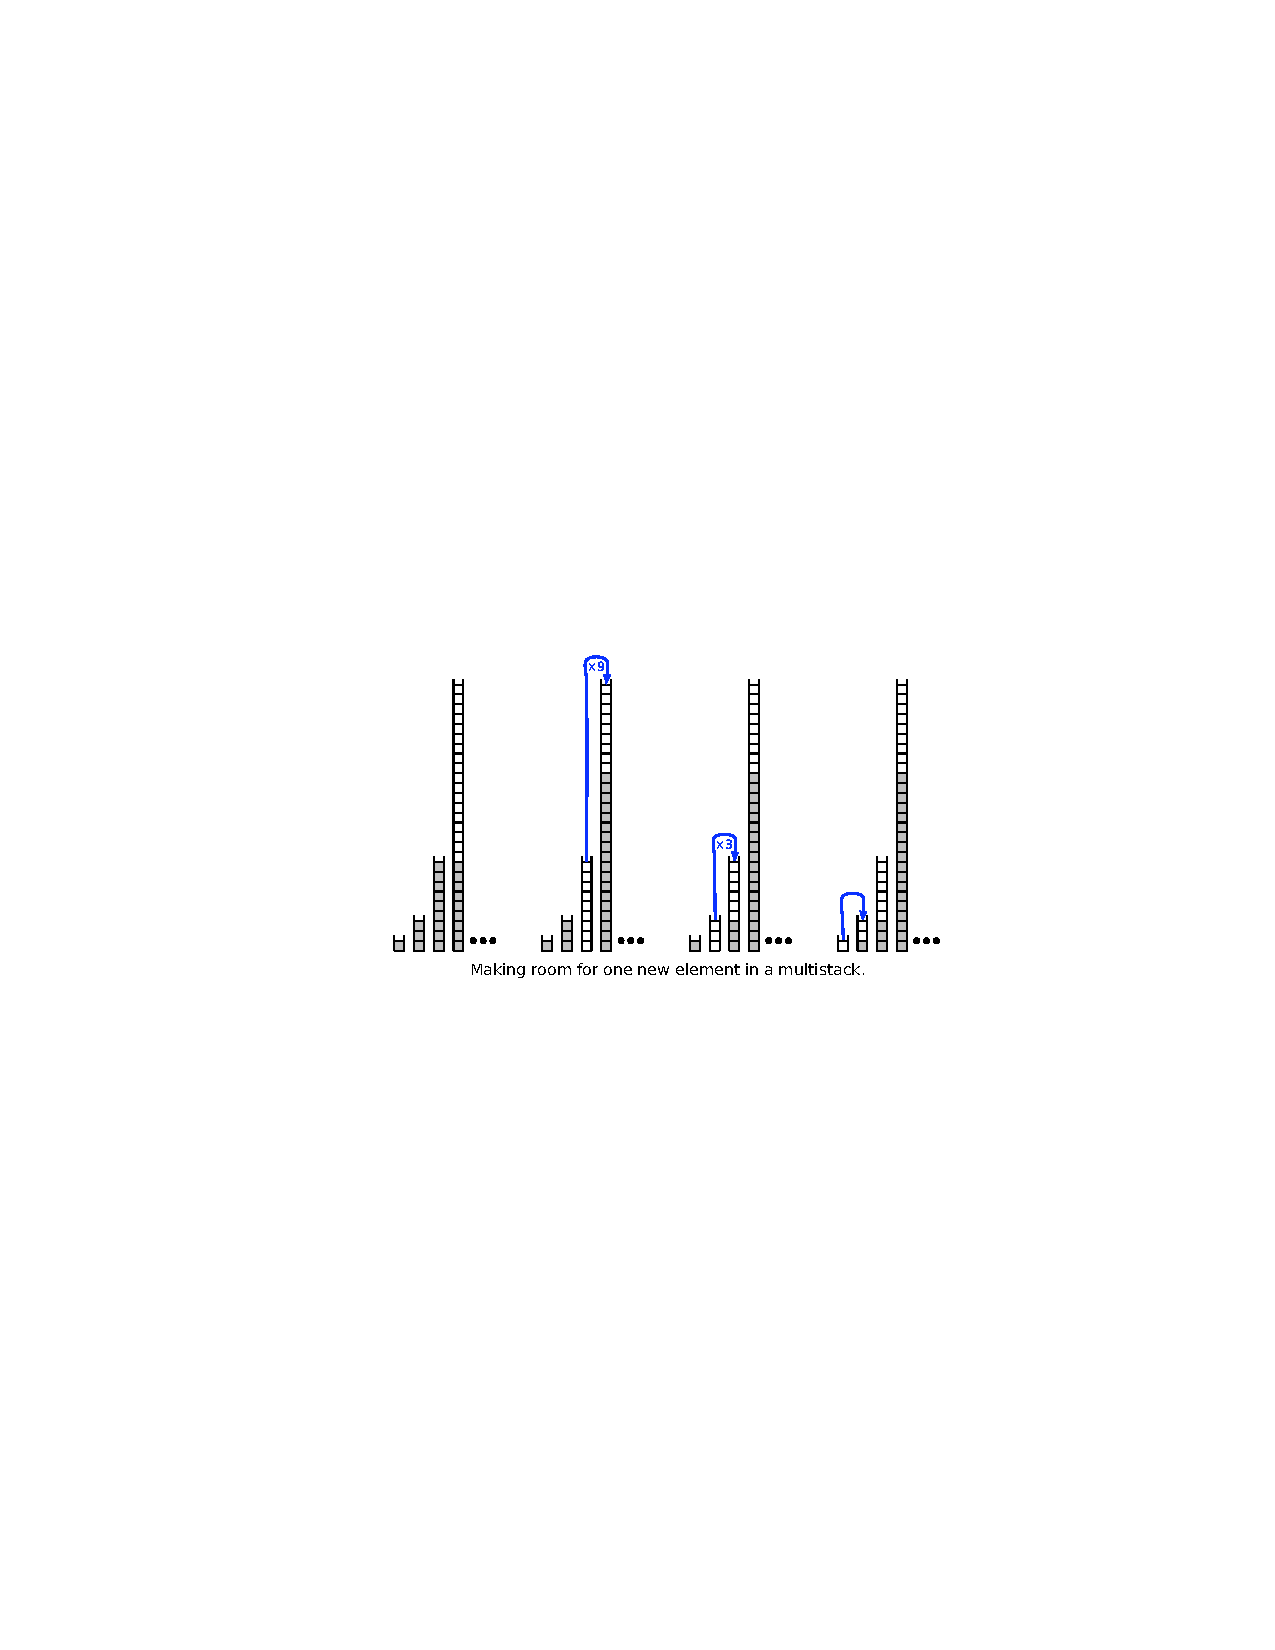
\includegraphics[width=0.5\textwidth]{Fig-MultiStack.pdf}
	\caption{An example of making room for one new element in a multistack.}
	\label{Fig-MultiStack}
	\end{figure}

    \begin{enumerate}
        \item In the worst case, how long does it take to push a new element onto a multistack containing $n$ elements?
        \item Prove that the amortized cost of a push operation is $O(\log n)$ by \emph{Aggregation Analysis}.
        \item {\color{red}(Optional Subquestion with Bonus)} Prove that the amortized cost of a push operation is $O(\log n)$ by \emph{Potential Method}.
    \end{enumerate}
    \begin{enumerate}
    \item
    \begin{solution}
    In the worst case, every stack in the multistack is full, so we need to move every element from the current stack to the next stack. Since there are totally $n$ elements, it takes $O(n)$ time to push a new element onto a multistack containing $n$ elements under this circumstance.
    \end{solution}

    \item
    \begin{proof} First we can implement the first few push operations manually to find the pattern of the time cost. The time cost table of the first few push operation is as follows.

    \begin{table}[htbp]
     	\footnotesize
     	\centering
     	\label{reduction}
     	\renewcommand\arraystretch{1.1}
     	\begin{tabular}{ccccccccccccccccccccc}
     		\hline
            \textbf{Push Count} & 1 & 2 & 3 & 4 & 5 & 6 & 7 & 8 & 9 & 10 & 11 & 12 & 13 & 14 & 15 & 16 & 17 & 18 & $\cdots$ \\ \hline
            \textbf{Inserting Cost} & 1 & 1 & 1 & 1 & 1 & 1 & 1 & 1 & 1 & 1 & 1 & 1 & 1 & 1 & 1 & 1 & 1 & 1 & $\cdots$ \\
            \textbf{Moving Stack 1 Cost} & & $3^0$ & $3^0$ & $3^0$ & $3^0$ & $3^0$ & $3^0$ & $3^0$ & $3^0$ & $3^0$ & $3^0$ & $3^0$ & $3^0$ & $3^0$ & $3^0$ & $3^0$ & $3^0$ & $3^0$ & $\cdots$ \\
            \textbf{Moving Stack 2 Cost} & & & & & $3^1$ & & & $3^1$ & & & $3^1$ & & & $3^1$ & & & $3^1$ & & $\cdots$ \\
            \textbf{Moving Stack 3 Cost} & & & & & & & & & & & & & & $3^2$ & & & & & $\cdots$ \\
            \textbf{$\cdots$} & & & & & & & & & & & & & & & & & & & $\cdots$ \\ \hline
            \textbf{Total Time Cost} & 1 & 2 & 2 & 2 & 5 & 2 & 2 & 5 & 2 & 2 & 5 & 2 & 2 & 14 & 2 & 2 & 5 & 2 & $\cdots$ \\
            \hline
     	\end{tabular}
        \end{table}

        Analyze the table above we can easily derive the following pattern:
        \begin{itemize}
        \item In every push operation, it will take $O(1)$ time to insert the new element.
        \item The time complexity of moving stack $k$ is $O(3^{k-1})$;
        \item Let $C_k(n)$ denote the total count of moving stack $k$ in the first $n$ push operations. Then $C_k(n)$ can be represented as follows.
        \begin{displaymath}
        C_k(n) = \left\lfloor \frac{\max(n - \sum_{i=0}^{k-1} 3^i, 0)}{3^{k-1}} \right\rfloor
        \end{displaymath}
        \end{itemize}
        Therefore, the total time complexity of the first $n$ operations is as follows.

        \begin{displaymath}
        \begin{aligned}
        T(n) &= n \times 1 + \sum_{k=1}^{\left\lfloor \log_3{(2n+1)} \right\rfloor}C_k(n) \cdot 3^{k-1} \\
             &= n + \sum_{k=1}^{\left\lfloor \log_3{(2n+1)} \right\rfloor}\left\lfloor \frac{\max(n - \sum_{i=0}^{k-1} 3^i, 0)}{3^{k-1}} \right\rfloor \cdot 3^{k-1} \\
             &\leq n + \sum_{k=1}^{\left\lfloor \log_3{(2n+1)} \right\rfloor}\left( \frac{n - \sum_{i=0}^{k-1} 3^i}{3^{k-1}} \right) \cdot 3^{k-1} \\
             &= n + \sum_{k=1}^{\left\lfloor \log_3{(2n+1)} \right\rfloor}{\left(n - \sum_{i=0}^{k-1} 3^i\right)} \\
             &= n + n \left\lfloor \log_3{(2n+1)} \right\rfloor - \sum_{k=1}^{\left\lfloor \log_3{(2n+1)} \right\rfloor} \frac{3^k - 1}{2} \\
             &= n + n \left\lfloor \log_3{(2n+1)} \right\rfloor + \frac{1}{2} \left\lfloor \log_3{(2n+1)} \right\rfloor - \frac{3^{\left\lfloor \log_3{(2n+1)} \right\rfloor} - 1}{4} + \frac{1}{2} \\
             &= O(n \log{n})
        \end{aligned}
        \end{displaymath}

        Notice that we use a property of floor function that $\left\lfloor X \right\rfloor \leq X$ in the derivations above. We can use another property $X-1 < \left\lfloor X \right\rfloor$ of floor function to get the lower bound of $T(n)$, which is also $\Omega(n \log{n})$. Therefore, $T(n) = \Theta(n \log{n})$.

        Hence, the amortized cost of one push operation is $O(\log{n})$
    \end{proof}

    \item
    \begin{proof}
        Let $num_j(S)$ denote number of elements in the $j$-th stack in the multistack for state $S$. Let $M$ denote the maximum number of stacks we need in multistack during $n$ push operations, and we can derive that $M = \left\lceil \log_3{(2n+1)} \right\rceil$. Then we define the potential function $\Phi(S)$ for state $S$ as follows.
        \begin{displaymath}
        \begin{aligned}
        \Phi(S) &\stackrel{\Delta}{=} \sum_{i = 1}^{M} {\sum_{j = 1}^i {num_j(S)}} \\
                &= \sum_{j=1}^{M} (M-j+1) num_j(S) \\
                &= (M+1) \sum_{j=1}^{M} num_j(S) - \sum_{j=1}^{M} j \cdot num_j(S)
        \end{aligned}
        \end{displaymath}

        Therefore, we have that $\Phi(S_i) \geq 0$ since $num_j(\cdot)$ is non-negative, and we can calculate that the potential function of initial state is $\Phi(S_0) = 0$. Thus, we meet the requirement of Potential Method, that is,
        \begin{displaymath}
        \Phi(S_i) \geq 0 = \Phi(S_0)
        \end{displaymath}

        For $i$-th operation, suppose it needs to move stack $1$, stack $2$, $\cdots$, and stack $k\ (k \leq M)$. Then we know that these stacks are all full, that is,
        \begin{displaymath}
        num_j(S_{i-1}) = 3^{j-1}, \quad j = 1,2,\cdots, k
        \end{displaymath}

        We can also calculate the time cost of this operation $c_i$ is as follows.
        \begin{equation}
        c_i = 1 + \sum_{j=1}^k 3^{j-1} = 1 + \frac{3^k - 1}{2} = \frac{3^k + 1}{2}
        \end{equation}

        Hence,
        \begin{equation}
        \begin{aligned}
        \hat{c_i} &= c_i + \Phi(S_i) - \Phi(S_{i-1}) \\
                  &= \frac{3^k + 1}{2} + \sum_{j=1}^M j \cdot (num_j(S_{i-1}) - num_j(S_i)) \\
                  &\stackrel{\Delta}{=} \frac{3^k + 1}{2} + T
        \end{aligned}
        \label{eq2-3-1}
        \end{equation}

        In the last step we let $T$ denote the summation $\sum_{j=1}^M j \cdot (num_j(S_{i-1}) - num_j(S_i))$. We will evaluate the change of $num_j(S)$ and try to simplify $T$ next.
        \begin{enumerate}
        \item For $j = 1$, we have $num_j(S_i) = 1$, because finally we will push an element to the first stack;
        \item For $1 < j \leq k$, we have $num_j(S_i) = num_{j-1}(S_{i-1})$, because we will move the elements in the $j$-th stack to the $(j+1)$-th stack;
        \item For $j = k+1$, we have $num_j(S_i) = num_j(S_{i-1}) + num_{j-1}(S_{i-1})$, because we will move the elements in the $k$-th stack to the $(k+1)$-th stack;
        \item For $k + 1 < j \leq M$, we have $num_j(S_i) = num_j(S_{i-1})$, because the operation does not involve in these stacks.
        \end{enumerate}

        Therefore, we can make some derivations to simplify $T$ as follows.
        \begin{displaymath}
        \begin{aligned}
        T &=  \sum_{j=1}^M j \cdot (num_j(S_{i-1}) - num_j(S_i)) \\
          &=  (M + 1) + \sum_{j=2}^{k+1} j \cdot (num_j(S_{i-1}) - num_j(S_i)) \\
          &=  (M + 1) -(k+1)\cdot num_k(S_{i-1}) + \sum_{j=2}^{k} j \cdot (num_j(S_{i-1}) - num_{j-1}(S_{i-1})) \\
          &=  (M + 1) -(k+1)\cdot 3^{k-1} + \sum_{j=2}^k j \cdot(3^{j-1} - 3^{j-2}) \\
          &=  (M + 1) -(k+1)\cdot 3^{k-1} + \sum_{j=1}^{k-1} (j+1)\cdot 3^j - \sum_{j=0}^{k-2} (j+2)\cdot 3^j \\
          &=  (M + 1) -(k+1)\cdot 3^{k-1} + k \cdot 3^{k-1} - 2 \cdot 3^0 - \sum_{j=1}^{k-2} 3^j \\
          &=  (M + 1) -3^{k-1} - 2 - \left( \frac{3^{k-1} - 1}{2} - 1 \right) \\
          &=  (M + 1) - \frac{3^k + 1}{2}
        \end{aligned}
        \end{displaymath}

        Plug the result of $T$ in Equation \eqref{eq2-3-1}, then we can continue calculating $\hat{c_i}$ as follows.
        \begin{equation}
        \begin{aligned}
        \hat{c_i} &= \frac{3^k + 1}{2} + T \\
                  &= \frac{3^k + 1}{2} + (M + 1) - \frac{3^k + 1}{2} \\
                  &= M + 1
        \end{aligned}
        \label{eq2-3-2}
        \end{equation}

        Therefore, with the help of Equation \eqref{eq2-3-2}, we can make some derivations as follows about the time cost of $n$ push operation $T(n)$.
        \begin{displaymath}
        \begin{aligned}
        \sum_{i=1}^n c_i &= \sum_{i=1}^n \hat{c_i} - \Phi(S_n) + \Phi(S_0)\\
                         &\leq \sum_{i=1}^n \hat{c_i}\\
                         &= n \cdot (M+1)\\
                         &= n \cdot \left(\left\lceil \log_3{(2n+1)} \right\rceil + 1\right) \\
                         &= O(n \log{n})
        \end{aligned}
        \end{displaymath}

        Hence, the amortized cost of one push operation is $O(\log{n})$

    \end{proof}
    \end{enumerate}	
    \clearpage


	\item Given a graph $G = (V, E)$, and let $V'$ be a strict subset of $V$. Prove the following propositions.
	
	\begin{enumerate}
		\item Let $T$ be a minimum spanning tree of a $G$. Let $T'$ be the subgraph of $T$ induced by $V'$, and let $G'$ be the subgraph of $G$ induced by $V'$. Then $T'$ is a minimum spanning tree of $G'$ if $T'$ is connected.
		\item Let $e$ be a minimum weight edge which connects $V'$ and $V \setminus V'$. There exists a minimum weight spanning tree which contains $e$.
	\end{enumerate}
    \begin{enumerate}
    \item
    \begin{proof}
    \textbf{(Contradiction)}  Assume that $V(G)$ denote the vertex set of graph $G$ and $E(G)$ denote the edge set of graph $G$. Let $w(e)$ denote the weight of edge $e$. Since the $T'$ is a connected subgraph of the spanning tree $T$ induced by $V'$, $T'$ must be a spanning tree of $G'$. Suppose the spanning tree $T'$ is not a minimum spanning tree of $G'$, then there exists a minimum spanning tree $T''$ of $G'$ satisfying that
    \begin{equation}
    \sum_{e \in E(T'')} w(e) < \sum_{e \in E(T')} w(e)
    \label{eq3-1}
    \end{equation}

    Suppose $T \setminus T'$ consists of $k$ \underline{connected} components $T_1, T_2, \cdots, T_k$, and each connected component $T_i\ (i = 1,2,\cdots,k)$ is the spanning tree of a subgraph $G_i$. Therefore the spanning tree $T$ and graph $G$ is constructed as follows (Fig.~\ref{fig3-1}).
    \begin{figure}[htbp]
      \centering
      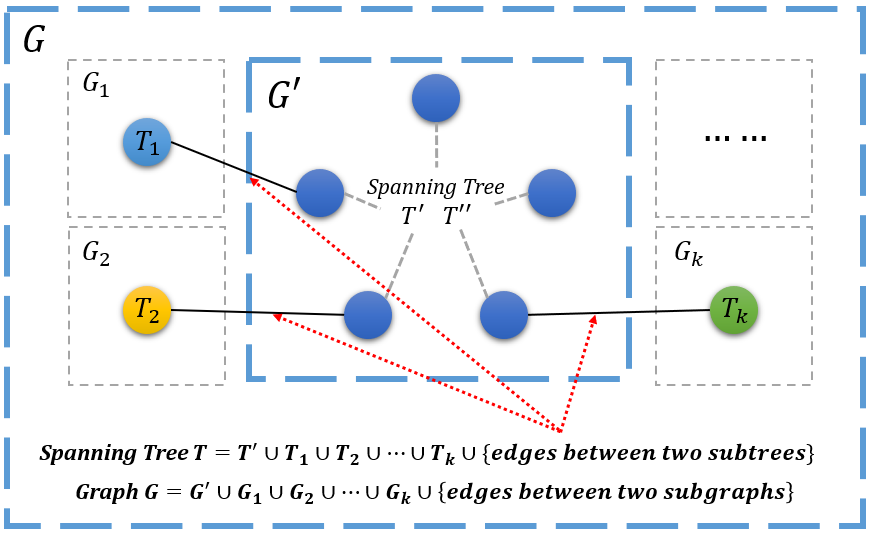
\includegraphics[width=5in]{prob3-1.png}\\
      \caption{The overview of the graph and spanning tree}\label{fig3-1}
    \end{figure}

    Therefore, graph $G$ is constructed by $(k + 1)$ subgraphs and edges between them and the spanning tree $T$ is constructed by $(k+1)$ spanning trees of the subgraphs and edges between $T_i$ and $T'$, since any two spanning trees $T_i$ and $T_j$ are not connected in $T \setminus T'$.

    Here is an important observation.
    \begin{center}
    \begin{minipage}[t]{0.8\linewidth}
    \begin{observation}
    For every spanning tree $T_i\ (i = 1,2,\cdots, k)$, there exists only one edge between $T_i$ and $T'$ in spanning tree $T$.
    \end{observation}
    \begin{proof}
        First, there must exist one edge between each $T_i$ and $T'$ in spanning tree $T$, otherwise $T_i$ and $T'$ will be disconnected in tree $T$ since any two spanning trees $T_i$ and $T_j$ are not connected in $T \setminus T'$, which is impossible. Second, there must exist only one such edge, otherwise it will form a cycle in spanning tree $T$, which is also impossible.
    \end{proof}
    \end{minipage}
    \end{center}

    Now let us consider a subgraph $T^* \stackrel{\Delta}{=} T'' \cup (T \setminus T')$. Basically we just replace $T'$ with $T''$ in spanning tree $T$, so $T^*$ includes all the vertices in graph $G$. Since the vertex sets of $T''$ and $T'$ are exactly the same, according to the observation, we can know that for every spanning tree $T_i\ (i = 1,2,\cdots, k)$, there exists only one edge between $T_i$ and $T''$ in spanning tree $T^*$. Thus, $T^*$ is a spanning tree of graph $G$.

    Let us evaluate the total weight of $T^*$. According to Equation \eqref{eq3-1}, we can make the following derivations.
    \begin{displaymath}
    \sum_{e \in E(T^*)} w(e) = \sum_{e \in E(T'')} w(e) + \sum_{e \in E(T \setminus T')} w(e) < \sum_{e \in E(T')} w(e) + \sum_{e \in E(T \setminus T')} w(e) = \sum_{e \in E(T)} w(e)
    \end{displaymath}

    Therefore, we have a spanning tree $T^*$ of graph $G$ whose total weight is less than the minimum spanning tree $T$ of graph $G$, which contradicts with the definition of minimum spanning tree.

    Hence, $T'$ is a minimum spanning tree of $G'$ if $T'$ is connected.
    \end{proof}

    \item
    \begin{proof}
    Assume that $V(G)$ denote the vertex set of graph $G$ and $E(G)$ denote the edge set of graph $G$. Suppose there is a spanning tree $T$ of graph $G$. If $e \in T$, then the proposition is proved. So let us consider the situation where edge $e$ is not in spanning tree $T$.

    We add edge $e$ into the spanning tree $T$ to form a new subgraph $T'$, that is,
    \begin{displaymath}
    V(T') = V(T), \quad E(T') = E(T) \cup \{e\}
    \end{displaymath}
    Notice that $T'$ is not a tree anymore because it \underline{has and only has} one cycle. Edge $e$ must be in the cycle, otherwise the cycle must already exist in $T$, which is impossible. Therefore, there exists another edge which connects $V'$ and $V \setminus V'$ in $T$ to complete the loop, say $e'$. Since $e$ is a minimum weight edge which connects $V'$ and $V \setminus V'$, we have that $w(e) \leq w(e')$.

    We put edge $e'$ out of the subgraph $T'$ to form a new subgraph $T^*$, that is,
    \begin{displaymath}
    V(T^*) = V(T'), \quad E(T^*) = E(T') \setminus \{e'\}
    \end{displaymath}
    Notice that $T^*$ is a spanning tree because it is a connected subgraph including all the vertex in graph $G$ and there is no cycle in $T^*$ anymore.

    Now let us focus on the relation between $w(e)$ and $w(e')$.
    \begin{itemize}
    \item If $w(e) < w(e')$, then we can make the following derivations.
    \begin{displaymath}
    \sum_{e^* \in E(T^*)} w(e^*) = w(e) + \sum_{e^* \in E(T)\setminus\{e'\}} w(e^*) < w(e') + \sum_{e^* \in E(T)\setminus\{e'\}} w(e^*) = \sum_{e^* \in E(T)} w(e^*)
    \end{displaymath}
    Thus, we have a spanning tree $T^*$ of graph $G$ whose total weight is less than the minimum spanning tree $T$ of graph $G$, which contradicts with the definition of minimum spanning tree. Therefore this situation cannot happen.
    \item If $w(e) = w(e')$, then we can make the following derivations.
    \begin{displaymath}
    \sum_{e^* \in E(T^*)} w(e^*) = w(e) + \sum_{e^* \in E(T)\setminus\{e'\}} w(e^*) = w(e') + \sum_{e^* \in E(T)\setminus\{e'\}} w(e^*) = \sum_{e^* \in E(T)} w(e^*)
    \end{displaymath}
    Thus, we have constructed another minimum spanning tree $T^*$ which includes edge $e$. Thus, the proposition is proved.
    \end{itemize}
    In summary, the proposition is proved.
    \end{proof}
    \end{enumerate}
\end{enumerate}



\textbf{Remark:} Please include your .pdf, .tex files for uploading with standard file names.


%========================================================================
\end{document}
